\documentclass[12pt]{article}
%%bzrcommit
\usepackage{amsmath,amsfonts,graphicx,cancel,boxedminipage,calc,etoolbox,nicefrac}

\usepackage[normalem]{ulem}

\makeatletter
\def\UL@putbox{\ifx\UL@start\@empty \else % not inner
  \vrule\@width\z@ \LA@penalty\@M
  {\UL@skip\wd\UL@box \UL@leaders \kern-\UL@skip}%
    \phantom{\box\UL@box}%
  \fi}
\makeatother

% for vertical centering
%\usepackage{array}
%\newcolumntype{M}{>{\centering\arraybackslash} m{.55\linewidth} }
%align table vertically to top

\usepackage[usenames,dvipsnames]{color}
\usepackage{tikz}
\tikzstyle{dashdotted}=              [dash pattern=on 3pt off 2pt on \the\pgflinewidth off 2pt]

\usetikzlibrary{arrows}
\usetikzlibrary{calc}

\setlength{\parskip}{1.2ex}    % space between paragraphs
\setlength{\parindent}{2em}    % amount of indention
\setlength{\textwidth}{175mm}      % default = 6.5"
\setlength{\oddsidemargin}{-5mm}   % default = 0"
\setlength{\textheight}{225mm}     % default = 9"
\setlength{\topmargin}{-7mm}      % default = 0"

  
\title{Introduction to Differential Equations}  
\author{Lake Bookman, Jack Bookman}    
\date{Monday, February 16, 2015}   

\providebool{showanswers}
\global\setbool{showanswers}{true}
\global\setbool{showanswers}{false}

\makeatletter\def\thetitle{\@title}\makeatother
\makeatletter\def\theauthor{\@author}\makeatother
\makeatletter\def\thedate{\@date}\makeatother

\providecommand{\makealttitle}
{
$$\;$$
\vspace{-4cm}
\textbf{
\begin{center}
\begin{LARGE}
\thetitle
\end{LARGE}
\\\vspace{4mm}
\begin{large}
\thedate
\end{large}
\end{center}
}
\hrule
\vspace{-.5cm}
$$\:$$
}

\providecommand{\makeblankold}[1]{\underline{\phantom{#1}}}
\providecommand{\makeblank}[1]{\uline{ \LARGE #1}}
\providecommand{\redtext}[1]{{\color{red} \bf  #1}}


\providecommand{\switchtext}[2]{%
\ifbool{showanswers}
	{%
		#1
	}%
	{%
		#2
	}%
}%

\providecommand{\privatetext}[1]{%
\ifbool{showanswers}
	{%
		\redtext{#1}
	}%
	{%
		\uline{ \LARGE #1}
	}%
}%

\providecommand{\privatetextnoblank}[1]{%
\ifbool{showanswers}
	{%
		\redtext{#1}
	}%
	{%
		 {\color{white} \uline{ \LARGE #1} }
	}%
}%

\providecommand{\privatetextnospace}[1]{%
\ifbool{showanswers}
	{%
		\redtext{#1}
	}%
	{%
	}%
}%

\providecommand{\alertbox}[2]
{
  \begin{center}
 \begin{boxedminipage}{.9\textwidth}
  \begin{tabular}{lcl}
\rule{1.5ex}{1.5ex} &
 \begin{minipage}{.883\textwidth}
 \vspace{1mm}
  \begin{center}\begin{large} \textbf{#1} \end{large}\\
#2
\end{center}
 \end{minipage}&\rule{1.5ex}{1.5ex}\end{tabular}
 \end{boxedminipage}
 \end{center}
}
\newlength{\mylen}

\providecommand{\ds}{\displaystyle}

\usetikzlibrary{positioning,arrows}

\begin{document}          
\makealttitle 
\setlength{\mylen}{0in}  
\vspace{-1.5cm} \\ 
\begin{enumerate}
\item
\begin{enumerate} 
\item  Is the point $x=1$, $y = 3$ (i.e. the point $(1,3)$ ) a solution to the equation $2 y + x = y + 4$?  Why? \vfill
\item  Is the point $(2,3)$ a solution to the equation $y^2 + x = y + 8$?  Why? \vfill
\item  Is the point $(1,1)$ a solution to the equation $x^2 + y^2 = 1$?  Why?\vfill
\item What does it mean that a point $(a,b)$ is a solution to an equation?  \vfill
\end{enumerate}
\item 
\begin{enumerate}
\item Is the function $y = x^2$ a solution to the equation $\frac{d y}{d x} = 2 x$ ? What about $y = x^2 + 5$? Why?\vfill
\item Is the function $y = -\frac{1}{x}$ a solution to the equation $\frac{ dy }{d x} =  y^2$?\\[2mm]
$\phantom{l}$ \hspace{1cm}  If $y = -\frac{1}{x}$, then $\frac{d y}{d x} =$  \privatetext{ $\frac{d}{dx} \left( - \frac{1}{x} \right)  = \frac{1}{x^2}$}\vspace{1cm}\\
$\phantom{l}$ \hspace{1cm}  If $y = -\frac{1}{x}$, then $y^2 =$  \privatetext{ $\frac{d}{dx} \left( - \frac{1}{x} \right)  = \frac{1}{x^2}$}\vspace{1cm}\\
$\phantom{l}$ \hspace{1cm}  If $y = -\frac{1}{x}$,  is $ \frac{d y}{d x} = y^2 $ ?  \vfill
\item Is the function $y = \frac{x^2}{2}$ a solution to the equation $\frac{ dy }{d x} =  y + x$?\\[2mm]
$\phantom{l}$ \hspace{1cm}  If $y = \frac{x^2}{2}$, then \hspace{2.8mm}$\frac{d y}{d x}\hspace{2.8mm} =\hspace{2.8mm}$  \privatetext{ $\frac{d}{dx} \left( - \frac{1}{x} \right)  = \frac{1}{x^2}$}\vspace{1cm}\\
$\phantom{l}$ \hspace{1cm}  If $y = \frac{x^2}{2}$, then $y + x =$  \privatetext{ $\frac{d}{dx} \left( - \frac{1}{x} \right)  = \frac{1}{x^2}$}\vspace{1cm}\\
$\phantom{l}$ \hspace{1cm}  If $y = \frac{x^2}{2}$,  is $ \frac{d y}{d x} = y + x $ ?  \vfill
\end{enumerate}
\newpage 
\item
\begin{enumerate}
\item Is the function $y = e^{3 x} $ a solution to the equation $\frac{ dy }{d x} = 3 y  $?\\[2mm]
$\phantom{l}$ \hspace{1cm}  If $y =  e^{3 x}$, then \hspace{0.0mm}$\frac{d y}{d x}\hspace{0.0mm} =\hspace{0.0mm}$  \privatetext{ $\frac{d}{dx} \left( - \frac{1}{x} \right)  = \frac{1}{x^2}$}\vspace{1cm}\\
$\phantom{l}$ \hspace{1cm}  If $y =  e^{3 x}$, then $3 y =$  \privatetext{ $\frac{d}{dx} \left( - \frac{1}{x} \right)  = \frac{1}{x^2}$}\vspace{1cm}\\

\item Is the function $y = e^{3 x} $ a solution to the equation $\frac{ dy }{d x} = 3 y  $?\\[2mm]
$\phantom{l}$ \hspace{1cm}  If $y =  e^{3 x}+1$, then \hspace{0.0mm}$\frac{d y}{d x}\hspace{0.0mm} =\hspace{0.0mm}$  \privatetext{ $\frac{d}{dx} \left( - \frac{1}{x} \right)  = \frac{1}{x^2}$}\vspace{1cm}\\
$\phantom{l}$ \hspace{1cm}  If $y =  e^{3 x}+1$, then $3 y =$  \privatetext{ $\frac{d}{dx} \left( - \frac{1}{x} \right)  = \frac{1}{x^2}$}\vspace{1cm}\\

\item Is the function $y = e^{3 x} $ a solution to the equation $\frac{ dy }{d x} = 3 y  $?\\[2mm]
$\phantom{l}$ \hspace{1cm}  If $y =  2e^{3 x}$, then \hspace{0.0mm}$\frac{d y}{d x}\hspace{0.0mm} =\hspace{0.0mm}$  \privatetext{ $\frac{d}{dx} \left( - \frac{1}{x} \right)  = \frac{1}{x^2}$}\vspace{1cm}\\
$\phantom{l}$ \hspace{1cm}  If $y =  2e^{3 x}$, then $3 y =$  \privatetext{ $\frac{d}{dx} \left( - \frac{1}{x} \right)  = \frac{1}{x^2}$}\vspace{1cm}\\
\end{enumerate}

\item Find a function that satisfies the differential equation $\frac{d y }{d x} = 3 x$. \vfill
Can you name another such function ? \vfill 
%\alertbox{}{
%\begin{minipage}{.8\textwidth}
%The equations of the form $\frac{dy}{dx} = y^2$ or $\frac{d y}{dx} = 2x $ are examples of differential equations.
%In fact, any equation of the form \privatetext{hello hello} is a \textbf{differential equation}.
%
%We say $y = f(t)$ is a 
%\end{minipage}}

\newpage
\item \begin{enumerate}
\item Express the following sentence as a differential equation (symbols instead of words): ``the rate of change of population is directly proportional to the size of the population." \vfill
\item Can you guess a function that satisfies the differential equation you wrote down in (a)? \vfill
\item Can you find another solution? \vfill
\end{enumerate}
 
\item Which of the following could be a solution to the simple immigration model with a growth rate of $2\%$ and an immigration rate of one hundred thousand people per year? Of those which are mathematical solutions, is there any reason to rule out such solutions?  ($P(t)$ is the population in millions)
\begin{enumerate}
\item $P(t) = -5 +4 e^{0.02 t} $ \vfill

\item $P(t) =5 + 10 e^{0.02 t}$ \vfill
\item $P(t) =-5 + 10 e^{0.02 t}$ \vfill
\item $P(t) =10 e^{0.02 t } - 5 t$  \vfill
\item $P(t) =5 e^{0.02 t } $\vfill
\end{enumerate}
\newpage
\item Both of the previous models allowed for the population to grow indefinitely, which may not be the most realistic idea. Yet the exponential model does a pretty decent job particularly when the population is reasonably small. For the next model, let's introduce the idea of the carrying capacity, $M$--a maximum allowed population Here we're going to try and write down a model which looks like the exponential model when $M$ is very large, limits growth of the population when $M$ is small.
\begin{enumerate}
\item Write a polynomial $f(x)$ such that $f(0) = 0$ and $f(M) = 0$. \vfill
\item Write a differential equation for the population where the rate of change is 0 when the population is $M$ (and when the population is 0). \vfill
\end{enumerate}

\item Below is a slope field for a differential equation very much like the one in the previous question. Sketch several solution curves on the graph below.\\
\begin{center}
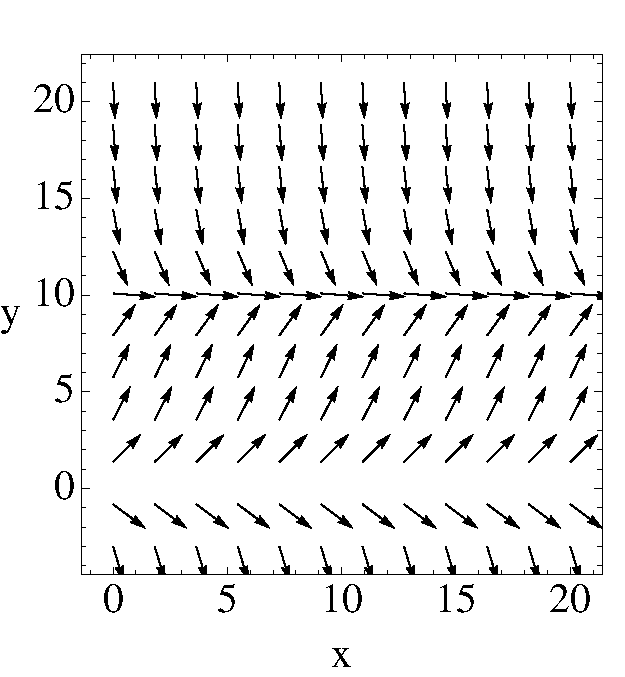
\includegraphics{simple_slope_field.pdf}
\end{center} \vfill
\end{enumerate}
\end{document}  
  
 
